
\section{Software Architecture}

\begin{frame}
\frametitle{Software Architecture}
The implementation of a functional architecture must consider several layers
of software architecture, where many implementation details affect the
performance of the system.\\
\vspace{0.2cm}
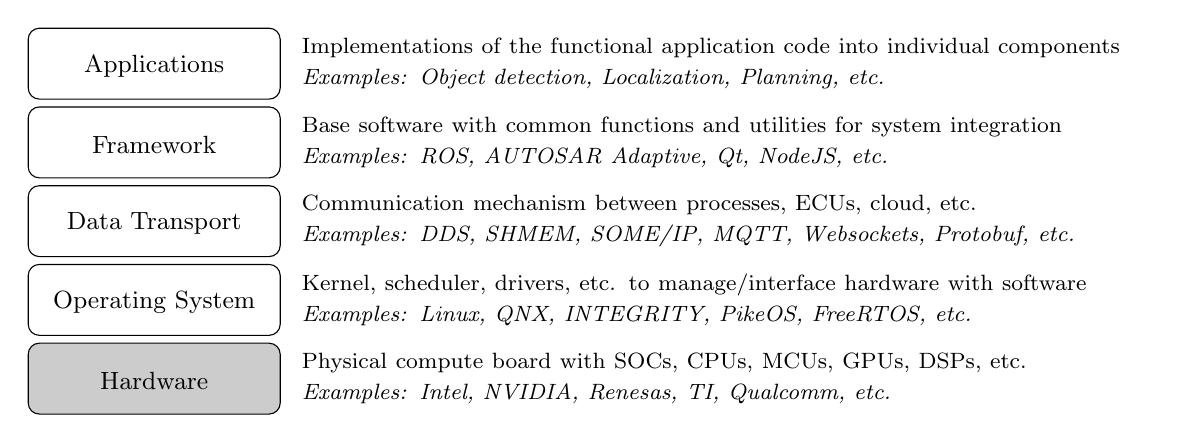
\begin{tikzpicture}[node distance=1cm,font=\small,
    layer/.style={
        draw=black,
        fill=white,
        rounded corners,
        minimum width=3.2cm,
        minimum height=0.9cm,
        text centered,
        text height=8pt},
    layerdark/.style={layer, fill=gray!40},
    ]
    \node[layer] (Apps) {Applications};
    \node[layer, below of=Apps] (FW) {Framework};
    \node[layer, below of=FW] (MW) {Data Transport};
    \node[layer, below of=MW] (OS) {Operating System};
    \node[layerdark, below of=OS] (HW) {Hardware};
    \node (AppsDesc) [right of=Apps, text width=10.75cm, xshift=6.25cm]{
        \footnotesize
        Implementations of the functional application code into individual
        components\\
        \emph{Examples: Object detection, Localization, Planning, etc.}
    };
    \node[right of=FW, text width=10.75cm, xshift=6.25cm] (FWDesc) {
        \footnotesize
        Base software with common functions and utilities for
        system integration\\
        \emph{Examples: ROS, AUTOSAR Adaptive, Qt, NodeJS, etc.}
    };
    \node[right of=MW, text width=10.75cm, xshift=6.25cm] (MWDesc) {
        \footnotesize
        Communication mechanism between processes, ECUs, cloud, etc.\\
        \emph{Examples: DDS, SHMEM, SOME/IP, MQTT, Websockets, Protobuf, etc.}
    };
    \node[right of=OS, text width=10.75cm, xshift=6.25cm] (OSDesc) {
        \footnotesize
        Kernel, scheduler, drivers, etc. to manage/interface hardware with
        software\\
        \emph{Examples: Linux, QNX, INTEGRITY, PikeOS, FreeRTOS, etc.}
    };
    \node[right of=HW, text width=10.75cm, xshift=6.25cm] (HWDesc) {
        \footnotesize
        Physical compute board with SOCs, CPUs, MCUs, GPUs, DSPs, etc.\\
        \emph{Examples: Intel, NVIDIA, Renesas, TI, Qualcomm, etc.}
    };
\end{tikzpicture}
\end{frame}

\begin{frame}
\frametitle{Software Frameworks for Autonomous Driving}
\framesubtitle{Framework requirements}
What are some of the functions, utilities and APIs that an application requires?
\vspace{0.25cm}
\begin{itemize}
    \item Concept of partitioning a larger system into components
    \item Means of receiving and transmitting data between components
    \item Configuration / parametrization of components
    \item Management of component execution und underlying CPU resources,
        e.g. threads
    \item Tools for development, debugging, and deployment
    \item Compatible with different programming languages and platforms
\end{itemize}
\end{frame}

\begin{frame}
\frametitle{Software Frameworks for Autonomous Driving}
\framesubtitle{Today's most popular solutions}
\centering
\begin{columns}[]
    \begin{column}{0.33\textwidth}
        \centering
        \includegraphics[width=0.8\textwidth]{images/logo_ros.png}\\
    \end{column}
    \begin{column}{0.33\textwidth}
        \centering
        \includegraphics[width=0.9\textwidth]{images/logo_mathworks.jpg}\\
    \end{column}
    \begin{column}{0.33\textwidth}
        \centering
        \includegraphics[width=0.3\textwidth]{images/logo_elektrobit.jpg}\\
    \end{column}
\end{columns}
\vspace{0.2cm}
\begin{columns}[]
    \begin{column}{0.33\textwidth}
        \centering
        \footnotesize
        Robot Operating System\footnotemark[1]\\
    \end{column}
    \begin{column}{0.33\textwidth}
        \centering
        \footnotesize
        MATLAB/Simulink\footnotemark[2]
    \end{column}
    \begin{column}{0.33\textwidth}
        \centering
        \footnotesize
        EB Assist ADTF\footnotemark[3]
    \end{column}
\end{columns}
\vspace{0.25cm}
\begin{columns}[]
    \begin{column}{0.33\textwidth}
        \centering
        \includegraphics[width=0.9\textwidth]{images/logo_autosar.png}\\
    \end{column}
    \begin{column}{0.33\textwidth}
        \centering
        \includegraphics[width=0.6\textwidth]{images/logo_nvidia.png}\\
    \end{column}
    \begin{column}{0.33\textwidth}
        \centering
        \includegraphics[width=0.8\textwidth]{images/logo_motionwise.png}\\
    \end{column}
\end{columns}
\vspace{0.2cm}
\begin{columns}[]
    \begin{column}{0.33\textwidth}
        \centering
        \footnotesize
        AUTOSAR\footnotemark[4]
    \end{column}
    \begin{column}{0.33\textwidth}
        \centering
        \footnotesize
        NVIDIA DriveWorks\footnotemark[5]
    \end{column}
    \begin{column}{0.33\textwidth}
        \centering
        \footnotesize
        TTTech Auto MotionWise\footnotemark[6]
    \end{column}
\end{columns}
\footnotetext[1]{\tiny{\url{https://ros.org/}}}
\footnotetext[2]{\tiny{\url{https://www.mathworks.com/products/automated-driving.html}}}
\footnotetext[3]{\tiny{\url{https://www.elektrobit.com/products/automated-driving/eb-assist/adtf/}}}
\footnotetext[4]{\tiny{\url{https://www.autosar.org/}}}
\footnotetext[5]{\tiny{\url{https://developer.nvidia.com/drive/driveworks}}}
\footnotetext[6]{\tiny{\url{https://www.tttech-auto.com/products/safety-software-platform/motionwise/}}}
\end{frame}

\begin{frame}
\frametitle{Software Frameworks for Autonomous Driving}
\framesubtitle{Today's most popular solutions}
\begin{center}
    \includegraphics[width=0.4\textwidth]{images/logo_apexai.png}
\end{center}
\vspace{0.25cm}
Apex.AI\footnotemark[1] has developed Apex.OS\footnotemark[2] and
Apex.Middleware\footnotemark[3], a software framework and
middleware based on ROS and designed for safety-certified automotive
applications.
\footnotetext[1]{\tiny{\url{https://www.apex.ai/}}}
\footnotetext[2]{\tiny{\url{https://www.apex.ai/apex-os}}}
\footnotetext[3]{\tiny{\url{https://www.apex.ai/apex-middleware}}}
\end{frame}

\subsection{ROS}

\begin{frame}
\frametitle{Robot Operating System (ROS)}
\framesubtitle{Overview}
\begin{columns}[]
    \begin{column}{0.7\textwidth}
        \begin{itemize}
            \item Most popular framework for developing robotics (and other)
                applications
            \item Open source with thousands of contributors world wide
            \item Widely adopted by universities, research institutes and
                and companies
            \item Thousands of packages\footnotemark[1] (applications) for
                sensors, perception, SLAM, motion planning, etc.
            \item Powerful suite of tools (visualization, introspection,
                debugging, etc.)
            \item Wide support for different programming languages
            \item Hundreds of autonomous vehicles in R\&D run on ROS
        \end{itemize}
    \end{column}
    \begin{column}{0.3\textwidth}
        \centering
        \includegraphics[width=\textwidth]{images/logo_ros.png}
    \end{column}
\end{columns}
\footnotetext[1]{\tiny{\url{https://index.ros.org/packages/}}}
\end{frame}

\begin{frame}
\frametitle{Robot Operating System (ROS)}
\framesubtitle{The basics}
\begin{columns}[]
    \begin{column}{0.5\textwidth}
        \begin{itemize}
            \item \textbf{Nodes}: A single processing entity with inputs and
                outputs
            \item \textbf{Topics}: Data channels between nodes
            \item \textbf{Messages}: The data type which is transmitted on a
                topic
            \item \textbf{Publisher}: Within a node, the entity that transmits
                data on a topic
            \item \textbf{Subscriber}: Within a node, the entity that receives
                data on a topic
            \item \textbf{Service}: Request/response mechanism between nodes
        \end{itemize}
    \end{column}
    \begin{column}{0.5\textwidth}
        \centering
        \includegraphics[width=\textwidth]{images/ros_overview.png}
        \tiny{Source: ROS 2 Tutorials - Understanding ROS 2 nodes\footnotemark[1]}
    \end{column}
\end{columns}
\footnotetext[1]{\tiny{\url{https://docs.ros.org/en/galactic/Tutorials/Understanding-ROS2-Nodes.html}}}
\end{frame}

\begin{frame}[fragile]
\frametitle{Robot Operating System (ROS)}
\framesubtitle{Example ROS 2 node in C++}
\tiny
\begin{minted}{cpp}
// From https://docs.ros.org/en/galactic/Tutorials/Writing-A-Simple-Cpp-Publisher-And-Subscriber.html
class MinimalPublisher : public rclcpp::Node {
    public:
        MinimalPublisher() : Node("minimal_publisher"), count_(0) {
            publisher_ = this->create_publisher<std_msgs::msg::String>("topic", 10);
            timer_ = this->create_wall_timer(500ms, std::bind(&MinimalPublisher::timer_callback, this));
        }
    private:
        void timer_callback() {
            auto message = std_msgs::msg::String();
            message.data = "Hello, world! " + std::to_string(count_++);
            RCLCPP_INFO(this->get_logger(), "Publishing: '%s'", message.data.c_str());
            publisher_->publish(message);
        }
        rclcpp::TimerBase::SharedPtr timer_;
        rclcpp::Publisher<std_msgs::msg::String>::SharedPtr publisher_;
        size_t count_;
};

int main(int argc, char * argv[]) {
    rclcpp::init(argc, argv);
    rclcpp::spin(std::make_shared<MinimalPublisher>());
    rclcpp::shutdown();
    return 0;
}
\end{minted}
\end{frame}

\begin{frame}
\frametitle{Robot Operating System (ROS)}
\framesubtitle{Tools}
ROS has a rich suite of tools, both included in the standard installation as
well as additional tools developed by the community.\\
Show the CLI, RViz, rqt, rosbag, etc.
\end{frame}

\subsection{Production Frameworks}

\begin{frame}
\frametitle{Production Software Frameworks}
Talk about how what is required to go from prototyping to a production
software architecture (Apex.OS, AUTOSAR, other --> name the properties
of such frameworks)
\end{frame}

\begin{frame}
\frametitle{AUTOSAR Classic}
\end{frame}

\begin{frame}
\frametitle{AUTOSAR Adaptive}
\end{frame}

\subsection{Middleware}

\begin{frame}
\frametitle{Data Transport Middlewares}
\framesubtitle{Overview}
\end{frame}

\begin{frame}
\frametitle{Data Transport Middlewares}
\framesubtitle{Shared memory}
\end{frame}

\begin{frame}
\frametitle{Data Transport Middlewares}
\framesubtitle{DDS}
\end{frame}

\begin{frame}
\frametitle{Data Transport Middlewares}
\framesubtitle{Automotive communication buses}
SOME/IP, CAN, Flexray
\end{frame}

\begin{frame}
\frametitle{Data Transport Middlewares}
\framesubtitle{MQTT}
\end{frame}

\subsection{Operating Systems}

\begin{frame}
\frametitle{Operating Systems}
Linux, QNX, INTEGRITY, PikeOS, EMCOS, etc. 
\end{frame}